\documentclass[a4paper,10pt,ngerman]{scrartcl}
\usepackage[ngerman]{babel}

\usepackage[T1]{fontenc}
\usepackage[utf8]{inputenc}
\usepackage[a4paper,margin=2.5cm]{geometry}

% Die nächsten drei Felder bitte anpassen:
\newcommand{\Name}{Laurenz Grote} % Teamname oder eigenen Namen angeben
\newcommand{\Einsendenummer}{Team 145 / Teilnahme 44325}
\newcommand{\Aufgabe}{Aufgabe 3: Dreiecke zählen}

% Aliase zum abdrucken von Shell-CMDs
\newcommand{\shellcmd}[1]{\texttt{\$ #1}\\}
\newcommand{\shellout}[1]{\texttt{#1}\\}

% Kopf- und Fußzeilen
\usepackage{scrlayer-scrpage}
\setkomafont{pageheadfoot}{\textrm}
\ifoot{\Name}
\cfoot{\thepage}
\chead{\Aufgabe}
\ofoot{\Einsendenummer}

% Für mathematische Befehle und Symbole
\usepackage{amsmath}
\usepackage{amsthm}
\usepackage{amssymb}
\newtheorem{definition}{Definition}[section]

% Für Bilder
\usepackage{graphicx}

% Für Algorithmen
\usepackage{algpseudocode}

% Für Quelltext
\usepackage{listings}
\usepackage{xcolor}
\definecolor{mygreen}{rgb}{0,0.6,0}
\definecolor{mygray}{rgb}{0.5,0.5,0.5}
\definecolor{mymauve}{rgb}{0.58,0,0.82}
\lstset{language={C++},
  keywordstyle=\color{blue},commentstyle=\color{mygreen},
  stringstyle=\color{mymauve},rulecolor=\color{black},
  basicstyle=\footnotesize\ttfamily,numberstyle=\tiny\color{mygray},
  captionpos=t, % sets the caption-position to bottom
  keepspaces=true, % keeps spaces in text
  numbers=left, numbersep=5pt, showspaces=false,showstringspaces=true,
  showtabs=false, stepnumber=1, tabsize=2, title=\lstname,
  literate=%
    {Ö}{{\"O}}1
    {Ä}{{\"A}}1
    {Ü}{{\"U}}1
    {ß}{{\ss}}1
    {ü}{{\"u}}1
    {ä}{{\"a}}1
    {ö}{{\"o}}1
}

% Für die Bibliographie
\usepackage[babel,german=quotes]{csquotes}
\usepackage[citestyle=authortitle-icomp]{biblatex}
\addbibresource{literatur.bib}

% Diese beiden Pakete müssen als letztes geladen werden
\usepackage{hyperref} % Anklickbare Links im Dokument

% Daten für die Titelseite
\title{\Aufgabe}
\author{\Name / \Einsendenummer}
\date{\today}

\begin{document}
\maketitle
\tableofcontents

\section{Lösungsidee}
Die Aufgabe habe ich so interpretiert, dass ein Dreieck aus drei beliebigen Strecken
gebildet wird.
Außerdem muss es über einen Flächeninhalt größer Null verfügen.
Dabei ist es irrelevant, ob das so gebildete Dreieck von einer
anderen Strecke durchtrennt wird.
Daher reicht es, drei Strecken jeweils isoliert zu betrachten.

Zur Lösung der Aufgabe habe ich diese anschließend in zwei Teilprobleme aufgeteilt:
\begin{itemize}
    \item[a] Dem Zusammenstellen aller möglichen Kombinationen aus drei Strecken
    \item[b] Der Überprüfung, ob eine Kombination zusammen ein Dreieck bildet
\end{itemize}

Problem a kann mit einer in der Umsetzung beschriebenen rekursiven Funktion gelöst werden.
Für Teilaufgabe b habe ich zunächst eine geeignete Definition von Dreiecken formuliert:
\begin{definition} \label{theo:dreiecke}
Drei Strecken bilden ein Dreieck,
wenn jede Strecke die jeweils anderen schneidet.
Die drei Schnittpunkte müssen verschieden sein,
sonst beträgt der Flächeninhalt Null.
\end{definition}

Um nun für Auswahlen von Strecken überprüfen zu können, ob sie auf die Definition 
zutreffen, müssen also Schnittpunkte berechnet werden.
Am effizientesten lassen sich Schnittpunkte mit Verfahren aus der Mathematik ermitteln.
Hierfür konvertiere ich die Strecken, die alle durch zwei Punkte definiert sind, in Geraden.

Zu beachten ist, dass nicht zu jeder Kombination von zwei Punkten eine lineare
Funktion existiert. Wenn beide Punkte die gleiche x-Koordinate teilen, entsteht eine zur
y-Achse parallele Senkrechte. Diese Senkrechten haben dann eine Funktionsgleichung von
\(x=n\).

Nachdem für alle Strecken durch sie verlaufende Geraden aufgestellt wurden, können
im späteren Programmablauf Schnittpunkte durch Gleich- oder Einsetzen ermittelt
werden. Anschließend muss aber immer überprüft werden, dass der Schnittpunkt sich
zwischen den die Strecke begrenzenden Punkten befindet. Außerdem gilt es zu überprüfen,
ob alle drei Punkte sich unterscheiden.

Alle Streckenauswahlen, auf die die Definition \ref{theo:dreiecke} zutrifft, bilden
ein Dreieck im Sinne der Aufgabenstellung.


\section{Umsetzung}
\subsection {Datenstruktur für Strecken / Geraden}
Zentral für die Lösungsidee ist eine effiziente Berechnung von Schnittpunkten
zwischen den Strecken.
Wie beschrieben werden dafür die Strecken in Geraden konvertiert.

Zu jeder möglichen Kombination aus zwei Punkten lässt sich wie beschrieben
entweder eine Gerade mit einer Funktionsgleichung vom Typen \(y=mx+n\) oder
eine Senkrechte parallel zur y-Achse mit einer Funktionsgleichung vom Typen \(x=n\)
bilden.
Bei letzterer entspricht  \(n\) dann logischerweise der gemeinsamen x-Koordinate.

Wenn eine lineare Funktion vom Typen \(y=mx+n\) aufgestellt wird,
kann deren Steigung \(m\) mit folgender Rechnung ermittelt werden:
\begin{equation}
    m=\frac{y_{P2} - y_{P1}}{x_{P2} - x_{P1}}
\end{equation}

Der y-Achsenabschnitt \(n\) ergibt sich aus folgender Rechnung:
\begin{equation}
    n=y_{P1} - x_{P1} \times m
\end{equation}

Die x- und y-Koordinaten des Anfangs- und Endpunktes einer jeden Strecke werden
in zwei Aggregaten\footnote{In der Programmiersprache C++ ist ein Aggregat eine
Möglichkeit der Sprache, verschiedene Variablen in einem Objekt zu bündeln.
Vorteil ist, dass der Konstruktor implizit und der Zugriff auf die Felder denkbar
einfach ist.} 
vom Typ \texttt{coord}\footnote{Coordinate} in einem Objekt der Klasse \texttt{line}
gespeichert.
Der Konstruktor dieser Klasse berechnet aus diesen beiden Punkten
wie oben dargestellt eine Geradengleichung.

Die Variablen \(m\) und \(n\) werden in entsprechenden Felder des Objektes notiert.
Um später feststellen zu können, ob es sich um lineare Funktion oder um eine Senkrechte 
handelt, wird außerdem der Bool \texttt{isLinearFunction\_} entsprechend gesetzt.

\subsection {Bilden der möglichen Streckenkombinationen}
\begin{wrapfigure}{r}{0.5\textwidth}
    \begin{tikzpicture}[every node/.style={draw,circle, minimum size=1cm}, scale=0.7]
    \node at (0, 7)     (R)         {\(\varnothing\)};

    \node at (2, 11)    (RO)        {\(\varnothing\)};
    \node at (2, 3)     (RA)        {1};

    \node at (4, 13)    (ROO)       {\(\varnothing\)};
    \node at (4, 9)     (ROB)       {2};
    \node at (4, 5)     (RAO)       {1};
    \node at (4, 1)     (RAB)       {1,2};
    
    \node at (6, 14)    (ROOO)      {\(\varnothing\)};
    \node at (6, 12)    (ROOC)      {3};
    \node at (6, 10)    (ROBO)      {2};
    \node at (6, 8)     (ROBC)      {2,3};
    \node at (6, 6)     (RAOO)      {1};
    \node at (6, 4)     (RAOC)      {1,3};
    \node at (6, 2)     (RABO)      {1,2};
    
    % Hervorgehobener Node
    \node[fill={rgb:red,1;green,2;blue,3}] at (6, 0) (RABC) 
        {\textcolor{white}{1,2,3}};
    
    \draw [-] (R) edge (RO) edge (RA);
    \draw [-] (RO) edge (ROO) edge (ROB) (RA) edge (RAB) edge (RAO);
    \draw [-] (ROO) edge (ROOO) edge (ROOC) (ROB) edge (ROBO) edge (ROBC);
    \draw [-] (RAO) edge (RAOO) edge (RAOC) (RAB) edge (RABO) edge (RABC);

    \node[draw=none] at (9, 7) (C) {\(\ldots\)};
\end{tikzpicture}

    \caption{Auswahl der Streckenkombinationen}
    \label{abb:streckrek}
\end{wrapfigure}
Um für jede mögliche Streckenkombination das Vorhandensein eines Dreiecks prüfen zu können, müssen alle möglichen Kombination zunächst einmal aufgestellt werden. Dies habe ich mithilfe einer rekursiven Funktion implementiert.

Ich habe den Streckenauswahlprozess als einen binären Baum interpretiert. Jede Strecke kann entweder Teil einer Auswahl sein -- oder eben auch nicht.

Die Auswahlfunktion wird zunächst mit einer leeren Menge als Auswahl aufgerufen.
Diese leere Menge bildet die Wurzel des Baumes.

Durch Auswahl oder Nicht-Auswahl der ersten Strecke ergeben sich zwei Mengen: Wieder eine
leere Menge (die erste Strecke wurde nicht ausgewählt) oder eine Menge mit der ersten
Strecke als Inhalt (die erste Strecke wurde ausgewählt).

In der nächsten Rekursionsstufe werden dann beide Mengen kopiert und den Kopien jeweils
die zweite Strecke hinzugefügt. Die Mengen nach den ersten drei Rekursionen habe ich
in Abbildung \ref{abb:streckrek} dargestellt.

Sobald eine Menge drei Strecken enthält, kann überprüft werden, ob die enthaltenen
Strecken ein Dreieck bilden.
Hierzu kann Definition \ref{theo:dreiecke} herangezogen werden.
Die genaue Umsetzung dieser Definition beschreibe ich in Abschnitt \ref{sec:eval}.

Wenn die Streckenauswahl ein Dreieck bildet, werden die Strecken in einem Vektor
gespeichert und an die nächsthöhere Rekursionsebene zurückgegeben.
Diese gibt dann wiederum einen Vektor über alle Dreiecksvektoren an die nächste Ebene
zurück.
Schlussendlich wird eine Liste über alle möglichen Dreiecke zurückgegeben.

\subsection{Streckenauswahlevaluation}
\label{sec:eval}
Zur Überprüfung einer Streckenauswahl auf das Bilden eines Dreiecks
müssen zunächst die Schnittpunkte zwischen den Strecken ermittelt werden.
Je nachdem, welchen Funktionstyp die Strecken haben,
müssen verschiedene Verfahren angewandt werden.

Zwischen zwei linearen Funktion lässt sich der Schnittpunkt folgendermaßen durch
Gleichsetzen ermitteln:

\begin{equation}
    \begin{aligned}
        m_1x+n_1 &= m_2x+n_2             &&\quad\vert -n_2          \\
        m_1x+n_1-n_2 &= m_2x             &&\quad\vert -m_1x         \\
        n_1-n_2 &= (m_2-m_1)x            &&\quad\vert \div(m_2-m_1) \\
        x &= \frac{n_1-n_2}{m_2-m_1}                                \\
        y &= m_1x+n_2                                               \\
    \end{aligned}
    \label{eq:linearschnitt}
\end{equation}

Der Schnittpunkt zwischen einer Geraden \(y=m_1x+n_1\) und einer Senkrechten \(x=n_2\),
liegt bei der y-Koordinate, die die Gerade an der x-Stelle der Senkrechten annimmt.
Zur Ermittlung dieses Wert muss also die Senkrechte in die Gerade eingesetzt werden:

\begin{equation}
    \begin{aligned}
        x &= n_2                    \\
        y &= m_1 \times x + n_1 \qquad\vert\ \text{einsetzen}  \\
        y &= m_1 \times n_2 + n_1   \\
    \end{aligned}
    \label{eq:senkrechtschnitt}
\end{equation}

Falls beide Funktionen Senkrechten sind, können sie sich nur schneiden,
wenn Start- oder Endpunkte sich überlappen.
Schließlich sind aufeinander liegende Strecken laut Aufgabenstellung ausgeschlossen.
Wenn Start- und Endpunkt zweier Senkrechten sich überlappen,
können diese beiden Senkrechten unmöglich gemeinsam mit einer Geraden
ein Dreieck bilden. Daher kann angenommen werden, dass eine Auswahl mit zwei Senkrechten
kein Dreieck bilden kann.\footnote{Den Sonderfall, dass zwei Senkrechten oder zwei Geraden
mit gleicher Steigung direkt aneinander grenzen und mit zwei weiteren Geraden ein Dreieck
bilden, beachte ich nicht, da diese beiden Strecken in der Eingabedatei als eine Strecke
angegeben werden könnten. Mit solchen Sonderfällen ist bei konstruierten Rätseln nicht
zu rechnen.}

\begin{wrapfigure}{r}{0.3\textwidth}
    \begin{center}
    \begin{tikzpicture}
    \draw (3,1) -- (1,1);
    \draw (2,2) -- (0,0);
    \draw (1,3) -- (1,1);
    
    \fill[red] (1,1) circle (.1cm);
\end{tikzpicture}

    \end{center}
    \caption{Dreieck mit der Flächengröße 0}
    \label{abb:dreieck}
\end{wrapfigure}
Abschließend muss für jeden Schnittpunkt geprüft werden,
ob er zwischen dem Start- und Endpunkt beider Strecken liegt.
Schließlich können die Geraden sich außerhalb der Strecken,
die nur ein Abschnitt der Geraden sind, schneiden.
Im Sinne der Aufgabenstellung zählen nur Schnittpunkte der Strecken.

Außerdem muss überprüft werden, dass die Schnittpunkte sich nicht gleichen.
Schließlich hätte das Dreieck sonst einen Flächeninhalt von Null.
Ein Beispiel für sich gleichende Schnittpunkte ist Abb. \ref{abb:dreieck}.

Obengenannte Rechnungen sind in der Geradenklasse \texttt{line} in der Funktion
\texttt{calculateIntersections} implementiert.
Je nachdem, welche Strecken der Funktion übergeben wurden,
führt sie die entsprechenden Rechnungen durch.
Die Funktion gibt ein \texttt{pair<bool, Coord>} zurück.
Wenn der Bool auf true steht,
ist im zweiten Feld des Paares ein Schnittpunkt vermerkt.
Ansonsten wurde kein Schnittpunkt gefunden.

In einer weiteren Funktion, \texttt{isOnLine(..)}, wird, sodenn
die Geraden sich schneiden, überprüft, ob die übergebene Koordinate zwischen
oder auf den die Strecke begrenzenden Punkten liegt.

Wenn alle Strecken sich wie oben beschrieben schneiden und die Schnittpunkte verschieden
sind, bilden die übergebenen Strecken ein Dreieck.

\subsection {Grafische Ausgabe}
Die grafische Ausgabe wurde mit HTML realisiert. Seit HTML5 kann SVG inline genutzt
werden.
Dies macht sich mein Programm zu nutze, indem es die Zeichnung und das Dreieck
als SVG-Objekte im HTML-Dokument ausgibt.
Den Ausgabecode habe ich aus Platzgründen nicht im Dokument aufgeführt.


\section{Beispiele}
Mein Programm erstellt neben der Ausgabe in das auf der BwInf-Seite genannte
Ausgabeformat auch einen grafischen Report im HTML-Format.
Dieser kann mit gängigen Browsern betrachtet werden.
Um Platz zu sparen, gebe ich an dieser Stelle für die BwInf-Beispiele nur die Anzahl
der gefundenen Dreicke wieder. Farbige grafische Ausgaben finden Sie im Einsendungszip.

Beispiel 3 wurde im Wettbewerbsverlauf ausgetauscht. Da mein Programm in der alten
Fassung ebenfalls 7 Dreiecke findet, gebe ich hier beide Fassungen an.

\begin{table}[h]
    \centering
    \begin{tabular}{l|lllllll}
        \textbf{Beispiel}           & 1 & 2 & 3 (alt) & 3 (neu) & 4 & 5 & 6 \\ \hline
        \textbf{gefundene Dreiecke} & 9 & 0 & 7       & 3 & 5 & 1 & 20
    \end{tabular}
    \caption{Offizielle Beispiele: gefundene Dreiecke}
    \label{tab:bwinfbeispiele}
\end{table}

Ich habe versucht, ein Beispiel mit allen möglichen Schnittpunkttypen zu konstruieren.
In diesem Beispiel findet mein Programm alle 4 Dreiecke.
Ausgaben finden Sie im Einsendungszip.

\begin{figure}[h]
\centering
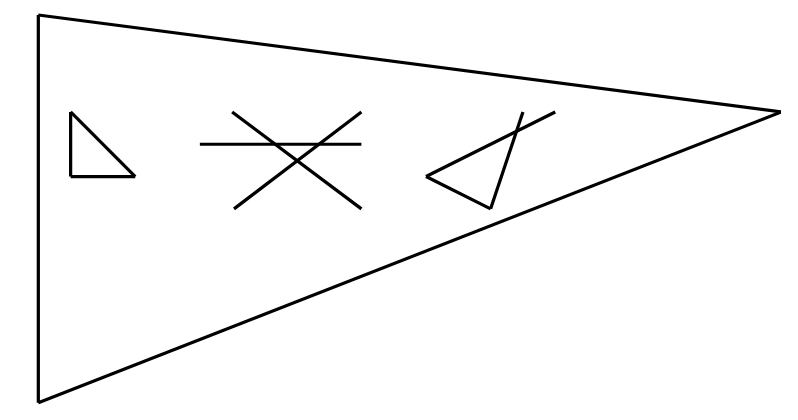
\includegraphics[width=0.7\textwidth]{eigbeispiel}
\caption{Eigenes Beispiel}
\end{figure}


\newpage
\section{Quellcode (ausschnittsweise)}
Augrund von Fehlern beim Rechnen mit Gleitkommazahlen muss immer mit einer
Fehlertoleranz gerechnet werden!

\lstinputlisting[label=lst:coordhpp, caption=Struktur einer Koordinate, firstline=4, lastline=10]{../Umsetzung/coord.hpp}
\lstinputlisting[label=lst:coordcpp, caption=Equals-Methode für Koordinaten, firstline=6, lastline=14]{../Umsetzung/coord.cpp}
\lstinputlisting[label=lst:linehpp, caption=Header für Geraden, firstline=8, lastline=35]{../Umsetzung/line.hpp}
\lstinputlisting[label=lst:linecpp, caption=Relevante Methoden der Geradenklasse, firstline=9, lastline=96]{../Umsetzung/line.cpp}
\lstinputlisting[label=lst:maincpp, caption=Hauptdatei, firstline=29, lastline=183]{../Umsetzung/main.cpp}


\nocite{*} % Alles REIN
\printbibliography[heading=bibintoc]%

\end{document}
